\documentclass[]{article}
\usepackage{lmodern}
\usepackage{amssymb,amsmath}
\usepackage{ifxetex,ifluatex}
\usepackage{fixltx2e} % provides \textsubscript
\ifnum 0\ifxetex 1\fi\ifluatex 1\fi=0 % if pdftex
  \usepackage[T1]{fontenc}
  \usepackage[utf8]{inputenc}
\else % if luatex or xelatex
  \ifxetex
    \usepackage{mathspec}
    \usepackage{xltxtra,xunicode}
  \else
    \usepackage{fontspec}
  \fi
  \defaultfontfeatures{Mapping=tex-text,Scale=MatchLowercase}
  \newcommand{\euro}{€}
\fi
% use upquote if available, for straight quotes in verbatim environments
\IfFileExists{upquote.sty}{\usepackage{upquote}}{}
% use microtype if available
\IfFileExists{microtype.sty}{%
\usepackage{microtype}
\UseMicrotypeSet[protrusion]{basicmath} % disable protrusion for tt fonts
}{}
\usepackage[margin=1in]{geometry}
\usepackage{color}
\usepackage{fancyvrb}
\newcommand{\VerbBar}{|}
\newcommand{\VERB}{\Verb[commandchars=\\\{\}]}
\DefineVerbatimEnvironment{Highlighting}{Verbatim}{commandchars=\\\{\}}
% Add ',fontsize=\small' for more characters per line
\usepackage{framed}
\definecolor{shadecolor}{RGB}{248,248,248}
\newenvironment{Shaded}{\begin{snugshade}}{\end{snugshade}}
\newcommand{\KeywordTok}[1]{\textcolor[rgb]{0.13,0.29,0.53}{\textbf{{#1}}}}
\newcommand{\DataTypeTok}[1]{\textcolor[rgb]{0.13,0.29,0.53}{{#1}}}
\newcommand{\DecValTok}[1]{\textcolor[rgb]{0.00,0.00,0.81}{{#1}}}
\newcommand{\BaseNTok}[1]{\textcolor[rgb]{0.00,0.00,0.81}{{#1}}}
\newcommand{\FloatTok}[1]{\textcolor[rgb]{0.00,0.00,0.81}{{#1}}}
\newcommand{\CharTok}[1]{\textcolor[rgb]{0.31,0.60,0.02}{{#1}}}
\newcommand{\StringTok}[1]{\textcolor[rgb]{0.31,0.60,0.02}{{#1}}}
\newcommand{\CommentTok}[1]{\textcolor[rgb]{0.56,0.35,0.01}{\textit{{#1}}}}
\newcommand{\OtherTok}[1]{\textcolor[rgb]{0.56,0.35,0.01}{{#1}}}
\newcommand{\AlertTok}[1]{\textcolor[rgb]{0.94,0.16,0.16}{{#1}}}
\newcommand{\FunctionTok}[1]{\textcolor[rgb]{0.00,0.00,0.00}{{#1}}}
\newcommand{\RegionMarkerTok}[1]{{#1}}
\newcommand{\ErrorTok}[1]{\textbf{{#1}}}
\newcommand{\NormalTok}[1]{{#1}}
\usepackage{graphicx}
\makeatletter
\def\maxwidth{\ifdim\Gin@nat@width>\linewidth\linewidth\else\Gin@nat@width\fi}
\def\maxheight{\ifdim\Gin@nat@height>\textheight\textheight\else\Gin@nat@height\fi}
\makeatother
% Scale images if necessary, so that they will not overflow the page
% margins by default, and it is still possible to overwrite the defaults
% using explicit options in \includegraphics[width, height, ...]{}
\setkeys{Gin}{width=\maxwidth,height=\maxheight,keepaspectratio}
\ifxetex
  \usepackage[setpagesize=false, % page size defined by xetex
              unicode=false, % unicode breaks when used with xetex
              xetex]{hyperref}
\else
  \usepackage[unicode=true]{hyperref}
\fi
\hypersetup{breaklinks=true,
            bookmarks=true,
            pdfauthor={Martin Cote},
            pdftitle={Exponential Distribution Investigation in R - Statistical Inference: Course Project - Question 1},
            colorlinks=true,
            citecolor=blue,
            urlcolor=blue,
            linkcolor=magenta,
            pdfborder={0 0 0}}
\urlstyle{same}  % don't use monospace font for urls
\setlength{\parindent}{0pt}
\setlength{\parskip}{6pt plus 2pt minus 1pt}
\setlength{\emergencystretch}{3em}  % prevent overfull lines
\setcounter{secnumdepth}{0}

%%% Use protect on footnotes to avoid problems with footnotes in titles
\let\rmarkdownfootnote\footnote%
\def\footnote{\protect\rmarkdownfootnote}

%%% Change title format to be more compact
\usepackage{titling}
\setlength{\droptitle}{-2em}
  \title{Exponential Distribution Investigation in R - Statistical Inference:
Course Project - Question 1}
  \pretitle{\vspace{\droptitle}\centering\huge}
  \posttitle{\par}
  \author{Martin Cote}
  \preauthor{\centering\large\emph}
  \postauthor{\par}
  \predate{\centering\large\emph}
  \postdate{\par}
  \date{April 26, 2015}


\usepackage{graphicx}


\begin{document}

\maketitle


\section{Overview}\label{overview}

This report provides a comparison between the values obtained directly
via the sample (and by the Central Limit Theorem) and to those of the
entire population.

\section{Required tools}\label{required-tools}

Loading the required libraries.

\section{Simulation}\label{simulation}

Preparing the simulation using: 1. num: number of exponentials per
simulations 2. lambda: the rate parameter used within this investigation
3. numsim: number of simulations used in this investigation

By: 1. running a `numsim' times the `rexp' (the ``random exponantial
distribution'') with a `lambda' rate for n=num. 2. saves the results
into matrix for further manipulation

\begin{Shaded}
\begin{Highlighting}[]
\CommentTok{# Number of averages}
\NormalTok{num <-}\StringTok{ }\DecValTok{40}
\CommentTok{# By default, our lambda value will be permanently set to 0.2}
\NormalTok{lambda <-}\StringTok{ }\FloatTok{0.2}

\CommentTok{# Number of simulations}
\NormalTok{numsim <-}\StringTok{ }\DecValTok{1000}

\CommentTok{# Simulating the random generation of an exponential distribution}
\NormalTok{simulateddata <-}\StringTok{ }\KeywordTok{matrix}\NormalTok{(}\DataTypeTok{data=}\KeywordTok{replicate}\NormalTok{(numsim, }\KeywordTok{rexp}\NormalTok{(}\DataTypeTok{n=}\NormalTok{num, }\DataTypeTok{rate=}\NormalTok{lambda)), }\DataTypeTok{nrow=}\NormalTok{numsim, }\DataTypeTok{ncol=}\NormalTok{num, }\DataTypeTok{byrow=}\OtherTok{TRUE} \NormalTok{)}
\end{Highlighting}
\end{Shaded}

\section{Sample Mean versus Theoretical
Mean}\label{sample-mean-versus-theoretical-mean}

Comparing the sample mean (i.e.~the mean for each rows) versus the
theoritical mean (i.e.~the mean for the entire simulation).

\begin{Shaded}
\begin{Highlighting}[]
\CommentTok{# Calculating the overall means}
\NormalTok{mns <-}\StringTok{ }\KeywordTok{rowMeans}\NormalTok{(simulateddata)}
\KeywordTok{mean}\NormalTok{(mns)}
\end{Highlighting}
\end{Shaded}

\begin{verbatim}
## [1] 5.000664
\end{verbatim}

\begin{Shaded}
\begin{Highlighting}[]
\CommentTok{# Calculating the mean}
\DecValTok{1} \NormalTok{/}\StringTok{ }\NormalTok{lambda}
\end{Highlighting}
\end{Shaded}

\begin{verbatim}
## [1] 5
\end{verbatim}

As observed, the sample mean calculated is fairly closed to the averages
of 40 means exponantials simulated, hence proving the CLT.

\begin{Shaded}
\begin{Highlighting}[]
\CommentTok{# Displaying the histogram of all simulated means of 40 random exponantials}
\KeywordTok{hist}\NormalTok{(mns, }\DataTypeTok{xlab=}\StringTok{"Means"}\NormalTok{, }\DataTypeTok{ylab=}\StringTok{"Frequency"}\NormalTok{, }\DataTypeTok{main=}\StringTok{"Sample Mean versus Theoritical Mean"}\NormalTok{)}
\CommentTok{#abline(v=mean(mns), col="blue", lwd=3)}
\KeywordTok{abline}\NormalTok{(}\DataTypeTok{v=}\DecValTok{1}\NormalTok{/lambda, }\DataTypeTok{col=}\StringTok{"red"}\NormalTok{, }\DataTypeTok{lwd=}\DecValTok{3}\NormalTok{)}
\end{Highlighting}
\end{Shaded}

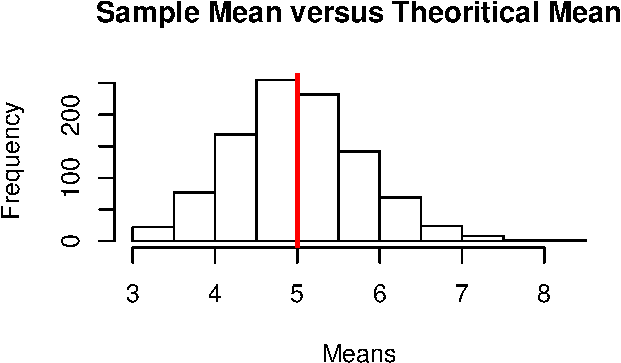
\includegraphics{statinference-courseproject-1-Question-1_files/figure-latex/unnamed-chunk-4-1.pdf}

The distribution is centered at or around both the sample mean or
theoritical mean.

\section{Sample Variance versus Theoretical
Variance}\label{sample-variance-versus-theoretical-variance}

Comparing the sample variance (i.e.~the variance for each rows) versus
the theoritical variance (i.e.~the variance for the entire simulation).

\begin{Shaded}
\begin{Highlighting}[]
\CommentTok{# Calculating the variances and averaging them:}
\NormalTok{vrs =}\StringTok{ }\OtherTok{NULL}
\NormalTok{for (i in }\DecValTok{1}\NormalTok{:numsim) \{}
  \NormalTok{vrs =}\StringTok{ }\KeywordTok{c}\NormalTok{(vrs, }\KeywordTok{var}\NormalTok{(simulateddata[i, ]))}
\NormalTok{\}}
\KeywordTok{mean}\NormalTok{(vrs)}
\end{Highlighting}
\end{Shaded}

\begin{verbatim}
## [1] 24.78703
\end{verbatim}

\begin{Shaded}
\begin{Highlighting}[]
\CommentTok{# Calculating the variance}
\NormalTok{(}\DecValTok{1} \NormalTok{/}\StringTok{ }\NormalTok{lambda)^}\DecValTok{2}
\end{Highlighting}
\end{Shaded}

\begin{verbatim}
## [1] 25
\end{verbatim}

As observed, the averages of all variances of the simulated 40 random
exponantials is fairly closed to the calculated variance, hence proving
the CLT.

\begin{Shaded}
\begin{Highlighting}[]
\KeywordTok{hist}\NormalTok{(vrs, }\DataTypeTok{xlab=}\StringTok{"Variances"}\NormalTok{, }\DataTypeTok{ylab=}\StringTok{"Frequency"}\NormalTok{, }\DataTypeTok{main=}\StringTok{"Sample Variance versus Theoritical Variance"}\NormalTok{)}
\KeywordTok{abline}\NormalTok{(}\DataTypeTok{v=}\NormalTok{(}\DecValTok{1}\NormalTok{/lambda)^}\DecValTok{2}\NormalTok{, }\DataTypeTok{col=}\StringTok{"red"}\NormalTok{, }\DataTypeTok{lwd=}\DecValTok{2}\NormalTok{)}
\end{Highlighting}
\end{Shaded}

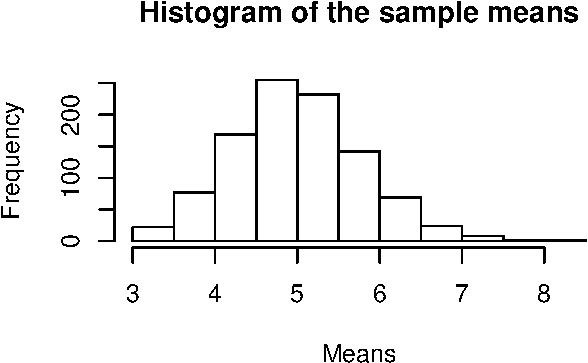
\includegraphics{statinference-courseproject-1-Question-1_files/figure-latex/unnamed-chunk-6-1.pdf}

The distribution is centered at or around both the sample variance or
the theoritical variance.

\section{Distribution}\label{distribution}

Investigating if the overall distribution is normal.

\begin{Shaded}
\begin{Highlighting}[]
\KeywordTok{hist}\NormalTok{(mns, }\DataTypeTok{xlab=}\StringTok{"Means"}\NormalTok{, }\DataTypeTok{ylab=}\StringTok{"Frequency"}\NormalTok{, }\DataTypeTok{main=}\StringTok{"Histogram of the sample means"}\NormalTok{)}
\end{Highlighting}
\end{Shaded}

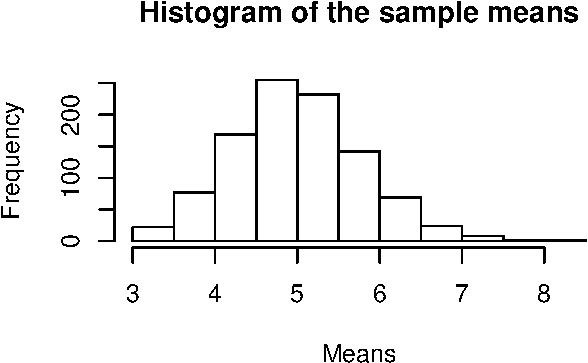
\includegraphics{statinference-courseproject-1-Question-1_files/figure-latex/unnamed-chunk-7-1.pdf}

Since the histogram follows/is closed to a normal distribution, we can
assume the distribution is approxamitively normal.

\end{document}
